\chapter{PCA}
\label{section:pca}

In this chapter we explain the derivation of PCA and the algorithm for compressing and decompressing the BTF.
We have chosen PCA for BTF compression, which belong to statistical methods, see Chapter \ref{section:stat_methods}.
While analytical methods and probabilistic methods have better compression ratio, they can produce worse rendering quality than PCA \cite{haindl}.



 \section{Derivation of PCA}
\label{section:derivation_pca}

Derivation of PCA can be done by means of a maximum variance formulation, as defined by Bishop \cite{Bishop}.
 Consider a set of variables $\left \{ x_{n} \right \}$, where $n=1..N$. $x_{n}$ are D-dimensional vectors. The aim is to project this data to an orthogonal basis while maximizing variation of new variables.
For the sake of simplicity, consider projection to one-dimensional space, i.e. to a new basis which consist of one vector $u_{1}$. 
As the magnitude of vector is not important in this case, let it be a unit vector, i.e. $u_{1}^Tu_{1}=1$.
 Then, each variable $x_{n}$ is projected onto a new basis, i.e. a scalar $u_{1}^Tx_{n}$.

 To compute the variance of the projected data, first we need to define the mean of projected data:

{\centering$\tfrac{1}{N}\sum_{n=1}^{N}u_{1}^Tx_{n}=u_{1}^T(\tfrac{1}{N}\sum_{n=1}^{N}x_{n})=u_{1}^T\overline{x}.$\\}

Then, the variance of the projected data looks the following way:

{\centering$\sum_{n=1}^{N}(u_{1}^Tx_{n}-u_{1}^T\overline{x} )^2=u_{1}^TSu_{1}$\\}

where $S$ is the covariance matrix defined as:

{\centering$S=\sum_{n=1}^{N}(x_{n}-\overline{x})(x_{n}-\overline{x})^T.$\\}

The next step is to maximize the variance $u_{1}^TSu_{1}$ with respect to $u_{1}$. In order to avoid $\left \| u_{1} \right \|$ growing to infinity, additional constrain has to be used,
i.e.  normalization constrain $u_{1}^Tu_{1}=1$.

Then, the problem looks the following way:

{\centering$maximize\,\,\,\,\,\,u_{1}^TSu_{1}$\\}

{\centering$\,\,\,\,\,subject \,\,to \,\,\,\,\,\,u_{1}^Tu_{1}=1$\\}

This can be solved with Lagrangian multiplier:

{\centering$u_{1}^TSu_{1}+\lambda_{1}(1-u_{1}^Tu_{1}).$\\}

By taking the derivative with respect to $u_{1}$ and setting it to zero, the local extremum can be found:

{\centering$\frac{\partial }{\partial u_{1}}u_{1}^TSu_{1}-\lambda_{1}\frac{\partial }{\partial u_{1}}u_{1}^Tu_{1}=0.$\\}

The result of taking derivative will be the following equation \cite{Bishop}:

{\centering$Su_{1}=\lambda_{1}u_{1}$\\}

which implies that this is an eigenvector and an eigenvalue problem, where $u_{1}$ is the eigenvector and $\lambda_{1}$ is the eigenvalue.
So, the maximum will be when eigenvector $u_{1}$ will have the largest eigenvalue $\lambda_{1}$. 
Then, such vector $u_{1}$ will be a \emph{principal component}.

In the same way it is possible to define the rest of principal components, 
which maximize the variance of projected data and with a condition that new components are orthogonal to other components.
After all, PCA involves evaluating the mean $\overline{x}$ and covariance matrix $S$ and finding eigenvectors with corresponding eigenvalues. 

 \section{SVD as PCA}
\label{section:svd}
Consider a set of variables $x_{n}$ be columns of matrix $X$. To compute covariance matrix $S$, matrix $X$ has to be centred, i.e. 

{\centering$X_{c}=X-1\overline{x}$\\}

where $\overline{x}$ is the vector of column-averages of matrix $X$ and matrix $1$ is the matrix of ones.
Then, the covariance matrix can be calculated the following way:

{\centering$S=X_{c}X_{c}^T$\\}


In practice to find eigenvectors and eigenvalues of covariance matrix S can be done by means of \emph{singular value decomposition}(SVD).
SVD does not require $S$ to be computed, instead it is enough to perform SVD on matrix $X_{c}$.
For any real matrix $X_{c}$ there is exist a decomposition \cite{svd}:

{\centering $X_{c}=U\Sigma V^{T}$ \\}

where $U$ and $V$ orthogonal matrices and $S$ diagonal matrix consisting of singular values.
The diagonal values of $\Sigma$ are the square roots of the eigenvalues of $X_{c}X_{c}^T$ \cite{Lecture12A}.
Consider SVD of $X_{c}X_{c}^T$:

{\centering $X_{c}X_{c}^T=(U\Sigma V^{T})(U\Sigma V^{T})^T$ \\}

{\centering $X_{c}X_{c}^T=(U\Sigma V^{T})(V\Sigma U)$ \\}

{\centering $V^{T}V=I$ \\}

{\centering $X_{c}X_{c}^T=U\Sigma^2 U^{T}$ \\}

From eigen decomposition theorem \cite{eigendecompostion} it is implied that matrix $U$ hold orthogonal eigenvectors of $X_{c}X_{c}^T$
and $\Sigma$ contains square roots of the eigenvalues.
Thus, decomposition of $X_{c}=U\Sigma V^{T}$ gives eigenvectors and eigenvalues needed for PCA.
\section{Algorithm}
\label{section:algorithm_step}
The algorithm of PCA for BTF compression and decompression is mainly borrowed from  Borshukov  \emph{et. al.} \cite[Ch.\ 15]{gpu_gems}.
We apply PCA per camera direction, which is why it can be called PCA RF. 
We also experimented and applied PCA per several directions at once.

\subsection{Compression}
\label{section:compression}
In the \emph{first} step of compression algorithm we built ABRDF representation of the BTF data.
Let matrix $A$ denote the stored BTF data.
We consider each image $I$ as three column vectors $a_{i}$ (red, green, and blue channels), where $i=0..(3*N)$. $N$ is the total number of images in BTF dataset and 3 is the number of channels per image.
The size of $a_{i}$ is $W\times H$, where $W$ and $H$ are dimensions of the image.
So, the matrix $A$ has the following dimensions $(W*H)\times(3*N)$, which consist of such columns $a_{i}$.
Rows of matrix $A$ are ABRDF representation of BTF, which will be dimensionally reduced.

The  \emph{second} step is called "centring" of the data. We compute the average value of each row of matrix $A$

{\centering $m_i=\frac{1}{3N}\sum_{i=1}^{3N}A_{i,j}$ \\}

Then, we subtract mean vector from each column of matrix $A$

{\centering $B_{i,j}=A_{i,j}-m_i.$ \\}

At the \emph{last} step, we compute singular value decomposition (SVD) of matrix $B$. The result of which will be the following decomposition

{\centering $B=U\Sigma V^{T}$ \\}

where matrix $U$ holds \emph{principal components} of size $W\times H$. $\Sigma$ is a diagonal matrix and holds the "importance" value of each principal components, and
matrix $V$ stores weights that are needed for reconstructing matrix $B$.

\subsection{Decompression}
\label{section:decompression}
The decompression step is simply matrix operations, which require to combine 3 matrices $U$, $\Sigma$, $V$ and mean vector $m$.
To make it a bit easier to decompress on GPU we construct new matrices as Borshukov  \emph{et. al.}

{\centering $L=\begin{bmatrix}
 m\mid U \Sigma
\end{bmatrix}$ \\}

{\centering $
R=\begin{bmatrix}
 1 ... 1   \\ 
  \, \, \, V^{T}
\end{bmatrix}.$ \\}
  Matrix $A$ takes such form of decompression $A=LR$. In detail, to decompress texture with index $i$ for first $C$ components, we do it separately for each color channel


{\centering $red(x,y)=\sum_{k=1}^{C}L_{xy,k}R_{k,3i+0}$ \\}
{\centering $green(x,y)=\sum_{k=1}^{C}L_{xy,k}R_{k,3i+1}$ \\}
{\centering $blue(x,y)=\sum_{k=1}^{C}L_{xy,k}R_{k,3i+2}$ \\}


\section{Angular Interpolation}
\label{chapter:interpolation}


BTF data is measured for a discrete set of light and camera directions, thus it is necessary to perform an interpolation to find the color value for unmeasured directions.
We propose a 2-D linear interpolation using barycentric weights \cite{haindl_visual}. 


Before computing interpolation weights for input direction $P$, it is required to find closest measured directions to it.
The determination of three closest directions is described in Chapter \ref{chapter:finding_triangle}. 
After three closest directions $P_{1}P_{2}P_{3}$ are known for input direction $P$, interpolation weights have to be computed.

 It is assumed that sampled measured directions form a convex hull, and found closest directions, i.e a triangle lies on the sampled hemisphere, as in Figure \ref{fig:acquisition_example}.
 Thus, it is possible to use barycentric coordinates to compute interpolation weights $w_{1},w_{2},w_{3}$.
  Chapter \ref{chapter:barycentric} explains how to compute barycentric coordinates.
  
To compute the final interpolated color we combine interpolation weights of light and camera directions.
Assume that $I$ and $O$ are input light and camera directions. 
Then, bounding triangles for both of them are $I_{1}I_{2}I_{3}$ and $O_{1}O_{2}O_{3}$ accordingly.
Corresponding barycentric weights then are $b_{i}=[b_{i1},b_{i2},b_{i3}]^T$ and $b_{o}=[b_{o1},b_{o2},b_{o3}]^T$.
The final color is the linear combination of $b_{i}$, $b_{o}$ weights and known measured color values 

 {\centering $ C_{f}=\sum_{u=1}^{3}b_{iu}\sum_{v=1}^{3}b_{ov}C_{uv},$\\} where $C_{uv}$ is a color value that corresponds for a light direction $I_{u}$ and a camera direction $O_{v}$.

\subsection{Finding Closest Directions}
\label{chapter:finding_triangle}
Depending on the material sampling, either uniform or non-uniform, different strategies can be applied for finding the closest directions for an input angle.
One of the strategies is to compute it in real-time each time or precomputed and stored in a cubemap \cite{haindl}.

BTF Bonn database \cite{btfBonn} provides the data with uniform sampling per longitude and per latitude. Depending on the longitude position, different quantization step is applied.
For areas closer to the bottom of the hemisphere quantisation step for latitude gets increased.
This is done to have relatively equal distance between the directions for any longitude position.
Also, more dense sampling needed at important areas (e.g. specular peak areas) to avoid interpolation artifacts. \cite{haindl}.

 Assume, a set of quantisation steps $S=\left \{ (\Delta \theta*n , \Delta \phi_n ) \mid n \in M \subseteq \mathbb{N} \right \}$, where $M$ specifies the number of steps.
For $\theta=0^{\circ}$ only one image is taken, i.e for $(0^{\circ},0^{\circ})$ direction.
  
First, we find four closest directions, and then decrease it three directions.
Let the direction for which we need to find the closest direction will be denoted as P=$(\theta^p, \phi^p)$.
To find closest points for $\theta^p$, we use algorithm described in Figure \ref{fig:findBound}.


\begin{figure}[h]
 \centering
 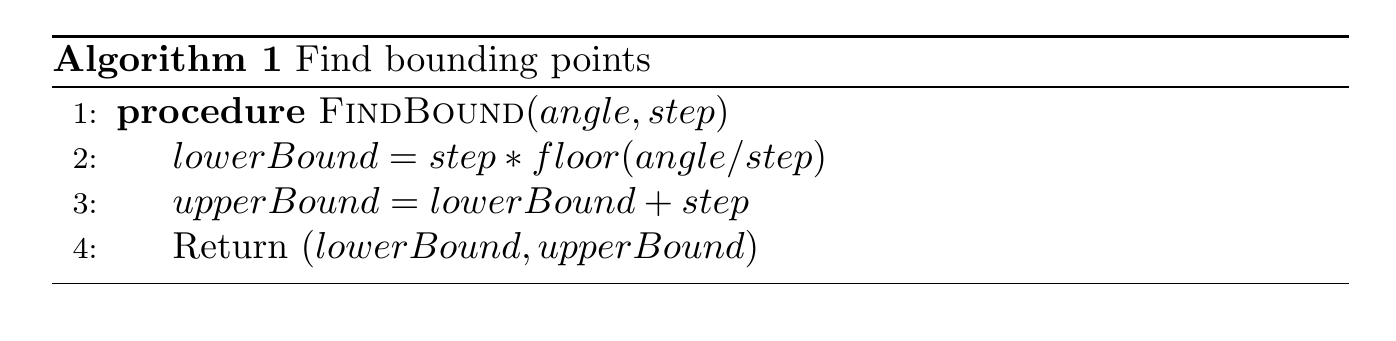
\includegraphics[width=1.0\textwidth]{figures/findBound}
 \caption[Finding Bounds ] {
 	{\bf Finding Bounds}

	}
 \label{fig:findBound}
\end{figure} 

We get that $(\theta_{L},\theta_{U})=FindBound(\theta_p,\Delta \theta)$. 
Because, the sampling steps are different for specific $\theta$, first we find closest points that lie at longitude $\theta_{L}$.
In the same manner as for $\theta$, i.e. $(\phi_{L}^1,\phi_{U}^1)=FindBound(\phi_p,\Delta \phi_n)$, where $n=\tfrac{\theta_L}{\Delta \theta}$.
And, finally for $\theta_{U}$ we get $(\phi_{L}^2,\phi_{U}^2) =FindBound(\phi_p,\Delta \phi_{n+1})$.

So, resulting four close directions to direction $P$ are: $A=(\theta_{L},\phi_{L}^1)$, $B=(\theta_{L},\phi_{U}^1)$, $C=(\theta_{U},\phi_{L}^2)$ and $D=(\theta_{U},\phi_{U}^2)$, as shown in Figure \ref{fig:triangle}.

We, then reduce to three closest directions, so then less weights would be computed.



\begin{figure}[h]
 \centering
 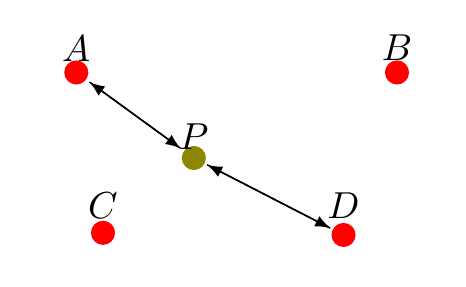
\includegraphics[width=.75\textwidth]{figures/triangle}
 \caption[Closest Directions ] {
 	{\bf Closest Directions}

	}
 \label{fig:triangle}
\end{figure} 
Consider, Figure \ref{fig:triangle}, which shows an example of four close directions.
Our aim is to find to which three directions $P$ is closer. 

One of the possible ways to find closest three directions is to compute a distance between $P$ and all other four directions and discard the furtherest one.
However, this is computational heavy for real-time.
The less computational demanding way could be to find approximately to which triangle direction $P$ belongs, i.e. $ABC$ or $CBD$.
The following method produces unnoticeable difference of visual results compared to the method which tests if the point $P$ belong to $ABC$ or $CBD$.


We compute to which direction $P$ is closer,i.e. whether to $A$ or $D$. A distance is computed as for Cartesian coordinates, but variables are changed for spherical coordinates: 
$x=rsin(\theta)cos(\phi)$, $y=rsin(\theta)sin(\phi)$, $z=rcos(\theta)$. So, the distance then will be:


{\centering$d=\sqrt{(x-x^{'})^2+(y-y^{'})^2+(z-z^{'})^2}=
\sqrt{r^2+r^{'2}-2rr'({\color{blue} sin(\theta)sin(\theta^{'})}{\color{magenta}cos(\phi)cos(\phi^{'})}+{\color{blue} sin(\theta)sin(\theta^{'})}{\color{magenta} sin(\phi)sin(\phi^{'})}+cos(\theta)cos(\theta^{'}))}=
\sqrt{r^2+r^{'2}-2rr'({\color{blue} sin(\theta)sin(\theta^{'})}{\color{magenta}cos(\phi-\phi^{'})}+cos(\theta)cos(\theta^{'}))}$\\}


Note that, in practice $r$ and $r^{'}$ are equal 1 for simplicity. As, we are interested in comparing distances, it is only enough to compare this term: 

{\centering$d^{'}=sin(\theta)sin(\theta^{'})cos(\phi-\phi^{'})+cos(\theta)cos(\theta^{'})$\\}

The bigger term  $d^{'}$, the smaller the overall distance, because there is are negative sign in the formula $d$. 
So, if $P$ is closer to $A$, the resulting three directions are $A$, $B$, $C$.
If $P$ closer to $D$ then $B$, $C$, $D$.

If the input direction $P$ is beyond the measuring directions, i.e. $\theta_p>\Delta \theta*n$ for any $n$.
In this case, we take two closer measured directions, i.e.  $A=(\theta_{L},\phi_{L}^1)$ and $B=(\theta_{L},\phi_{U}^1)$ and perform linear interpolation between these two directions.




\subsection{Barycentric Coordinates}
\label{chapter:barycentric}
Common interpolation technique for a BTF is barycentric coordinates interpolation. 
However, it is computational heavy, so the following approximation algorithm proposed by Hatka and Haindl \cite{btfblender} will be used.

Assume that a triangle $P_{1}P_{2}P_{3}$ bounds input point P, for which we want to compute interpolation weights. 
Figure \ref{fig:acquisition_example} demonstrates the hemisphere on which triangle $P_{1}P_{2}P_{3}$ lies.
$C_{P}$ denotes desired pixel color. 
So, generally speaking linearly interpolation of that pixel will be $C_{P}=w_{1}C_{P1} + w_{2}C_{P2} + w_{1}C_{P2}$, 
where $C_{P1},C_{P2},C_{P3}$ correspond to color values of the found triangle $P_{1}P_{2}P_{3}$. Weights $w_{1},w_{2},w_{3}$ are normalized and sum up to $1$.

Weights  $w_{1},w_{2},w_{3}$ defined as volumes $V_{1},V_{2},V_{3}$ which correspond to $PP_{2}P_{3}O$, $PP_{3}P_{1}O$, $PP_{1}P_{2}O$ tetrahedrons, where $O=(0,0,0)$.
 Volumes calculated as determinates of $4\times 4$ vectors

{\centering $w_{1}:=V_{1}=\frac{1}{6}\left | det(PP_{2}P_{3}O) \right |$ \\}
{\centering $w_{2}:=V_{2}=\frac{1}{6}\left | det(PP_{3}P_{1}O) \right |$ \\}
{\centering $w_{3}:=V_{3}=\frac{1}{6}\left | det(PP_{1}P_{2}O) \right |$ \\}

Last step is the normalization of found volumes, i.e. $V_{i}=\frac{V_{i}}{\sum_{i=1}^{3}V_{i}}$.
